Vyšetřili jsme závislost standardní odchylky šumového napětí na počtu sumací, výsledky jsou v grafu \ref{g:s} a tabulce \ref{t:s}. V grafu \ref{g:sum} je zakresleno několik spekter pro vybrané počty sumací (jsou vertikálně posunuté pro lepší porovnatelnost). Podle očekávání se intenzita šumu snižuje.

\begin{graph}[htbp] 
\centering
% GNUPLOT: LaTeX picture with Postscript
\begingroup
  \makeatletter
  \providecommand\color[2][]{%
    \GenericError{(gnuplot) \space\space\space\@spaces}{%
      Package color not loaded in conjunction with
      terminal option `colourtext'%
    }{See the gnuplot documentation for explanation.%
    }{Either use 'blacktext' in gnuplot or load the package
      color.sty in LaTeX.}%
    \renewcommand\color[2][]{}%
  }%
  \providecommand\includegraphics[2][]{%
    \GenericError{(gnuplot) \space\space\space\@spaces}{%
      Package graphicx or graphics not loaded%
    }{See the gnuplot documentation for explanation.%
    }{The gnuplot epslatex terminal needs graphicx.sty or graphics.sty.}%
    \renewcommand\includegraphics[2][]{}%
  }%
  \providecommand\rotatebox[2]{#2}%
  \@ifundefined{ifGPcolor}{%
    \newif\ifGPcolor
    \GPcolorfalse
  }{}%
  \@ifundefined{ifGPblacktext}{%
    \newif\ifGPblacktext
    \GPblacktexttrue
  }{}%
  % define a \g@addto@macro without @ in the name:
  \let\gplgaddtomacro\g@addto@macro
  % define empty templates for all commands taking text:
  \gdef\gplbacktext{}%
  \gdef\gplfronttext{}%
  \makeatother
  \ifGPblacktext
    % no textcolor at all
    \def\colorrgb#1{}%
    \def\colorgray#1{}%
  \else
    % gray or color?
    \ifGPcolor
      \def\colorrgb#1{\color[rgb]{#1}}%
      \def\colorgray#1{\color[gray]{#1}}%
      \expandafter\def\csname LTw\endcsname{\color{white}}%
      \expandafter\def\csname LTb\endcsname{\color{black}}%
      \expandafter\def\csname LTa\endcsname{\color{black}}%
      \expandafter\def\csname LT0\endcsname{\color[rgb]{1,0,0}}%
      \expandafter\def\csname LT1\endcsname{\color[rgb]{0,1,0}}%
      \expandafter\def\csname LT2\endcsname{\color[rgb]{0,0,1}}%
      \expandafter\def\csname LT3\endcsname{\color[rgb]{1,0,1}}%
      \expandafter\def\csname LT4\endcsname{\color[rgb]{0,1,1}}%
      \expandafter\def\csname LT5\endcsname{\color[rgb]{1,1,0}}%
      \expandafter\def\csname LT6\endcsname{\color[rgb]{0,0,0}}%
      \expandafter\def\csname LT7\endcsname{\color[rgb]{1,0.3,0}}%
      \expandafter\def\csname LT8\endcsname{\color[rgb]{0.5,0.5,0.5}}%
    \else
      % gray
      \def\colorrgb#1{\color{black}}%
      \def\colorgray#1{\color[gray]{#1}}%
      \expandafter\def\csname LTw\endcsname{\color{white}}%
      \expandafter\def\csname LTb\endcsname{\color{black}}%
      \expandafter\def\csname LTa\endcsname{\color{black}}%
      \expandafter\def\csname LT0\endcsname{\color{black}}%
      \expandafter\def\csname LT1\endcsname{\color{black}}%
      \expandafter\def\csname LT2\endcsname{\color{black}}%
      \expandafter\def\csname LT3\endcsname{\color{black}}%
      \expandafter\def\csname LT4\endcsname{\color{black}}%
      \expandafter\def\csname LT5\endcsname{\color{black}}%
      \expandafter\def\csname LT6\endcsname{\color{black}}%
      \expandafter\def\csname LT7\endcsname{\color{black}}%
      \expandafter\def\csname LT8\endcsname{\color{black}}%
    \fi
  \fi
  \setlength{\unitlength}{0.0500bp}%
  \begin{picture}(9070.00,5668.00)%
    \gplgaddtomacro\gplbacktext{%
      \csname LTb\endcsname%
      \put(1342,704){\makebox(0,0)[r]{\strut{} 0}}%
      \csname LTb\endcsname%
      \put(1342,1487){\makebox(0,0)[r]{\strut{} 0.0001}}%
      \csname LTb\endcsname%
      \put(1342,2270){\makebox(0,0)[r]{\strut{} 0.0002}}%
      \csname LTb\endcsname%
      \put(1342,3054){\makebox(0,0)[r]{\strut{} 0.0003}}%
      \csname LTb\endcsname%
      \put(1342,3837){\makebox(0,0)[r]{\strut{} 0.0004}}%
      \csname LTb\endcsname%
      \put(1342,4620){\makebox(0,0)[r]{\strut{} 0.0005}}%
      \csname LTb\endcsname%
      \put(1342,5403){\makebox(0,0)[r]{\strut{} 0.0006}}%
      \csname LTb\endcsname%
      \put(1474,484){\makebox(0,0){\strut{} 0}}%
      \csname LTb\endcsname%
      \put(2374,484){\makebox(0,0){\strut{} 0.1}}%
      \csname LTb\endcsname%
      \put(3274,484){\makebox(0,0){\strut{} 0.2}}%
      \csname LTb\endcsname%
      \put(4174,484){\makebox(0,0){\strut{} 0.3}}%
      \csname LTb\endcsname%
      \put(5074,484){\makebox(0,0){\strut{} 0.4}}%
      \csname LTb\endcsname%
      \put(5973,484){\makebox(0,0){\strut{} 0.5}}%
      \csname LTb\endcsname%
      \put(6873,484){\makebox(0,0){\strut{} 0.6}}%
      \csname LTb\endcsname%
      \put(7773,484){\makebox(0,0){\strut{} 0.7}}%
      \csname LTb\endcsname%
      \put(8673,484){\makebox(0,0){\strut{} 0.8}}%
      \put(176,3053){\rotatebox{-270}{\makebox(0,0){\strut{}$\sigma^2_{\bar{u^n}}$ ($\cdot 10^{-4}$)}}}%
      \put(5073,154){\makebox(0,0){\strut{}$1/\sqrt{N}$}}%
    }%
    \gplgaddtomacro\gplfronttext{%
      \csname LTb\endcsname%
      \put(3190,5230){\makebox(0,0)[r]{\strut{}naměřeno}}%
      \csname LTb\endcsname%
      \put(3190,5010){\makebox(0,0)[r]{\strut{}$\num{0.000691}/\sqrt{N}$}}%
    }%
    \gplbacktext
    \put(0,0){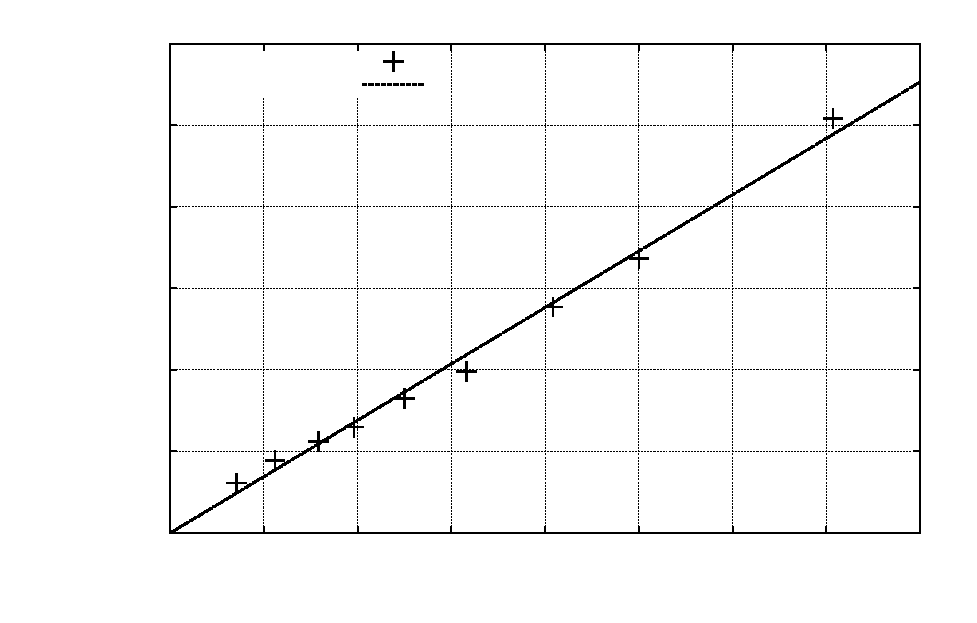
\includegraphics{s}}%
    \gplfronttext
  \end{picture}%
\endgroup

\caption{Závislost standardní odchylky šumového napětí na počtu sumací}
\label{g:s}
\end{graph}

\begin{tabulka}[htbp]
\centering
\begin{tabular}{cc}
$N$ & $\sigma^2_{\bar{u^n}}$ ($\cdot 10^{-4}$) \\\hline
2  & 5,079 \\
4 & 3,363 \\
6 & 2,772 \\
10 & 1,978 \\
16 & 1,651 \\
26 & 1,297 \\
40 & 1,119 \\
80 & 0,8890 \\
200 & 0,6124 \\
\end{tabular}
\caption{Závislost standardní odchylky šumového napětí na počtu sumací}
\label{t:s}
\end{tabulka}

\begin{graph}[htbp] 
\centering
% GNUPLOT: LaTeX picture with Postscript
\begingroup
  \makeatletter
  \providecommand\color[2][]{%
    \GenericError{(gnuplot) \space\space\space\@spaces}{%
      Package color not loaded in conjunction with
      terminal option `colourtext'%
    }{See the gnuplot documentation for explanation.%
    }{Either use 'blacktext' in gnuplot or load the package
      color.sty in LaTeX.}%
    \renewcommand\color[2][]{}%
  }%
  \providecommand\includegraphics[2][]{%
    \GenericError{(gnuplot) \space\space\space\@spaces}{%
      Package graphicx or graphics not loaded%
    }{See the gnuplot documentation for explanation.%
    }{The gnuplot epslatex terminal needs graphicx.sty or graphics.sty.}%
    \renewcommand\includegraphics[2][]{}%
  }%
  \providecommand\rotatebox[2]{#2}%
  \@ifundefined{ifGPcolor}{%
    \newif\ifGPcolor
    \GPcolortrue
  }{}%
  \@ifundefined{ifGPblacktext}{%
    \newif\ifGPblacktext
    \GPblacktextfalse
  }{}%
  % define a \g@addto@macro without @ in the name:
  \let\gplgaddtomacro\g@addto@macro
  % define empty templates for all commands taking text:
  \gdef\gplbacktext{}%
  \gdef\gplfronttext{}%
  \makeatother
  \ifGPblacktext
    % no textcolor at all
    \def\colorrgb#1{}%
    \def\colorgray#1{}%
  \else
    % gray or color?
    \ifGPcolor
      \def\colorrgb#1{\color[rgb]{#1}}%
      \def\colorgray#1{\color[gray]{#1}}%
      \expandafter\def\csname LTw\endcsname{\color{white}}%
      \expandafter\def\csname LTb\endcsname{\color{black}}%
      \expandafter\def\csname LTa\endcsname{\color{black}}%
      \expandafter\def\csname LT0\endcsname{\color[rgb]{1,0,0}}%
      \expandafter\def\csname LT1\endcsname{\color[rgb]{0,1,0}}%
      \expandafter\def\csname LT2\endcsname{\color[rgb]{0,0,1}}%
      \expandafter\def\csname LT3\endcsname{\color[rgb]{1,0,1}}%
      \expandafter\def\csname LT4\endcsname{\color[rgb]{0,1,1}}%
      \expandafter\def\csname LT5\endcsname{\color[rgb]{1,1,0}}%
      \expandafter\def\csname LT6\endcsname{\color[rgb]{0,0,0}}%
      \expandafter\def\csname LT7\endcsname{\color[rgb]{1,0.3,0}}%
      \expandafter\def\csname LT8\endcsname{\color[rgb]{0.5,0.5,0.5}}%
    \else
      % gray
      \def\colorrgb#1{\color{black}}%
      \def\colorgray#1{\color[gray]{#1}}%
      \expandafter\def\csname LTw\endcsname{\color{white}}%
      \expandafter\def\csname LTb\endcsname{\color{black}}%
      \expandafter\def\csname LTa\endcsname{\color{black}}%
      \expandafter\def\csname LT0\endcsname{\color{black}}%
      \expandafter\def\csname LT1\endcsname{\color{black}}%
      \expandafter\def\csname LT2\endcsname{\color{black}}%
      \expandafter\def\csname LT3\endcsname{\color{black}}%
      \expandafter\def\csname LT4\endcsname{\color{black}}%
      \expandafter\def\csname LT5\endcsname{\color{black}}%
      \expandafter\def\csname LT6\endcsname{\color{black}}%
      \expandafter\def\csname LT7\endcsname{\color{black}}%
      \expandafter\def\csname LT8\endcsname{\color{black}}%
    \fi
  \fi
  \setlength{\unitlength}{0.0500bp}%
  \begin{picture}(10204.00,7936.00)%
    \gplgaddtomacro\gplbacktext{%
      \csname LTb\endcsname%
      \put(198,704){\makebox(0,0)[r]{\strut{}}}%
      \csname LTb\endcsname%
      \put(198,2312){\makebox(0,0)[r]{\strut{}}}%
      \csname LTb\endcsname%
      \put(198,3920){\makebox(0,0)[r]{\strut{}}}%
      \csname LTb\endcsname%
      \put(198,5527){\makebox(0,0)[r]{\strut{}}}%
      \csname LTb\endcsname%
      \put(198,7135){\makebox(0,0)[r]{\strut{}}}%
      \csname LTb\endcsname%
      \put(330,484){\makebox(0,0){\strut{}-80}}%
      \csname LTb\endcsname%
      \put(922,484){\makebox(0,0){\strut{}-70}}%
      \csname LTb\endcsname%
      \put(1515,484){\makebox(0,0){\strut{}-60}}%
      \csname LTb\endcsname%
      \put(2107,484){\makebox(0,0){\strut{}-50}}%
      \csname LTb\endcsname%
      \put(2699,484){\makebox(0,0){\strut{}-40}}%
      \csname LTb\endcsname%
      \put(3292,484){\makebox(0,0){\strut{}-30}}%
      \csname LTb\endcsname%
      \put(3884,484){\makebox(0,0){\strut{}-20}}%
      \csname LTb\endcsname%
      \put(4476,484){\makebox(0,0){\strut{}-10}}%
      \csname LTb\endcsname%
      \put(5069,484){\makebox(0,0){\strut{} 0}}%
      \csname LTb\endcsname%
      \put(5661,484){\makebox(0,0){\strut{} 10}}%
      \csname LTb\endcsname%
      \put(6253,484){\makebox(0,0){\strut{} 20}}%
      \csname LTb\endcsname%
      \put(6845,484){\makebox(0,0){\strut{} 30}}%
      \csname LTb\endcsname%
      \put(7438,484){\makebox(0,0){\strut{} 40}}%
      \csname LTb\endcsname%
      \put(8030,484){\makebox(0,0){\strut{} 50}}%
      \csname LTb\endcsname%
      \put(8622,484){\makebox(0,0){\strut{} 60}}%
      \csname LTb\endcsname%
      \put(9215,484){\makebox(0,0){\strut{} 70}}%
      \csname LTb\endcsname%
      \put(9807,484){\makebox(0,0){\strut{} 80}}%
      \put(176,4187){\rotatebox{-270}{\makebox(0,0){\strut{}}}}%
      \put(5068,154){\makebox(0,0){\strut{}frekvence (\si{\kHz})}}%
    }%
    \gplgaddtomacro\gplfronttext{%
      \csname LTb\endcsname%
      \put(858,7498){\makebox(0,0)[r]{\strut{}200}}%
      \csname LTb\endcsname%
      \put(858,7278){\makebox(0,0)[r]{\strut{}26}}%
      \csname LTb\endcsname%
      \put(858,7058){\makebox(0,0)[r]{\strut{}6}}%
      \csname LTb\endcsname%
      \put(858,6838){\makebox(0,0)[r]{\strut{}2}}%
    }%
    \gplbacktext
    \put(0,0){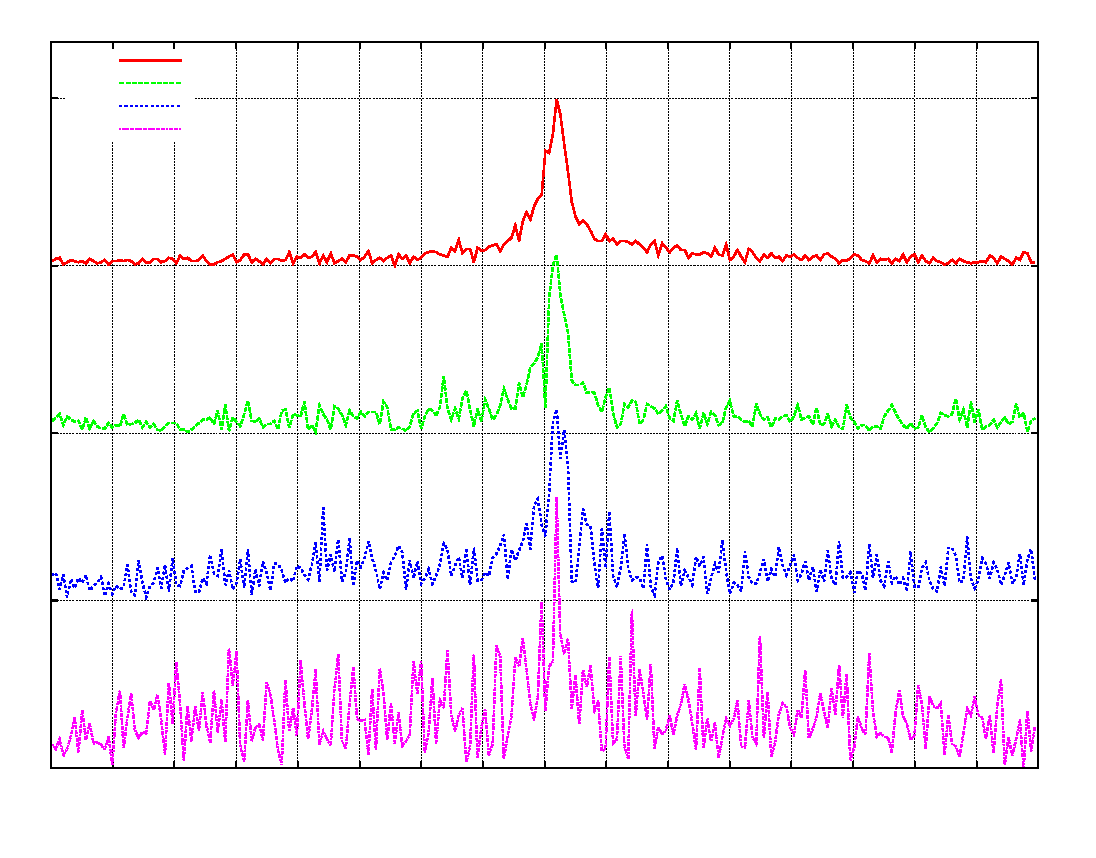
\includegraphics{sum}}%
    \gplfronttext
  \end{picture}%
\endgroup

\caption{Spektrum pro vybrané počty sumací.}
\label{g:sum}
\end{graph}